\paragraph{Placebo test plots:}  We developed a series of placebo test plots to investigate the statistical significance of the gap between the treatment and its synthetic control.  The series of plots below (Figures \ref{fig:ps50}, \ref{fig:ps20}, \ref{fig:ps10}, \ref{fig:ps5}, and \ref{fig:ps2}) show the implications of different thresholds for keeping control states in the placebo test.  The criterion for inclusion is the degree of difference between the pre-treatment (1981-85) MSPE for the placebo control gap vs. the gap for the treatment state.  We try a range from basically allowing all the states (50x) to a strict filter (2x).  The best compromise between allowing states to participate in the model and keeping out those with bad synthetic control is 10x (Figure \ref{fig:ps10}).  In that formulation the treatment state is relatively consistently below nearly all the placebo control states until the end of the period.  We discount the results towards the end of the treatment period because it is far beyond the support of the pre-treatment period.  These results indicate that there is very likely a significant decrease in fatalities from primary seatbelt laws.  

\begin{figure}[htbp]
\begin{center}
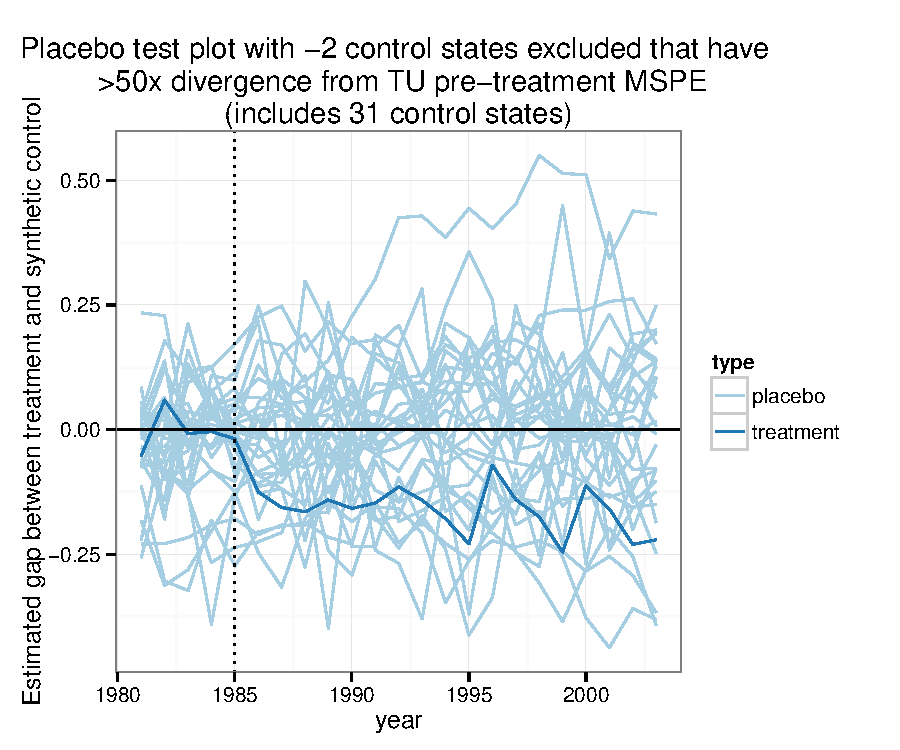
\includegraphics{img-placeboTest50.pdf}
\caption{Placebo test results comparing treatment with placebo analysis on all control states.  This plot does not exclude any states from the analysis.}
\label{fig:ps50}
\end{center}
\end{figure}

\begin{figure}[htbp]
\begin{center}
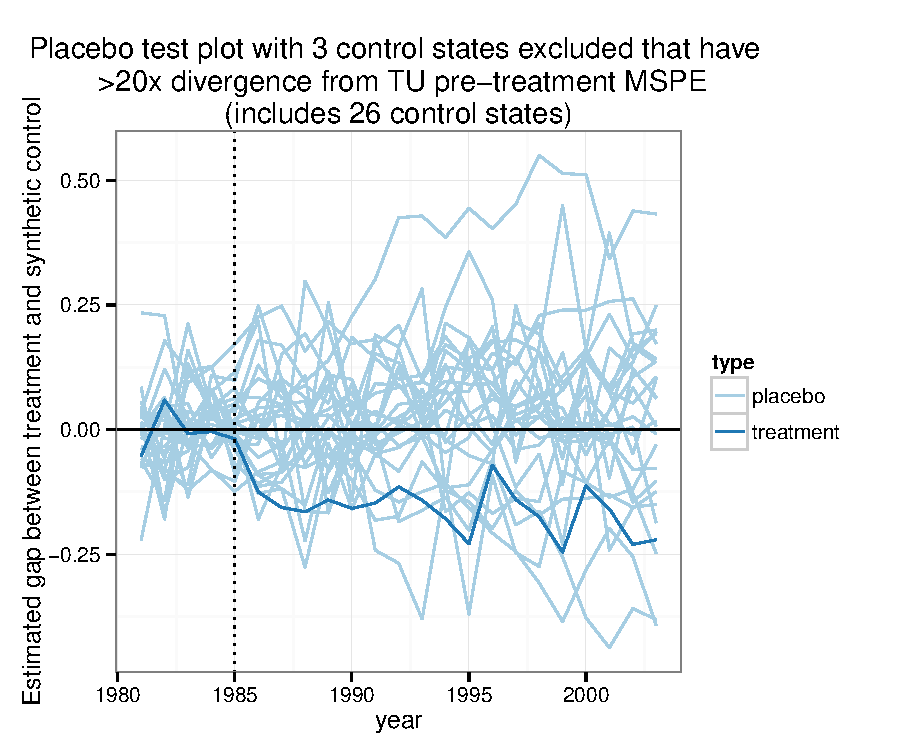
\includegraphics{img-placeboTest20.pdf}
\caption{Placebo test results comparing treatment with placebo analysis on all control states.  This plot excludes control states with MSPE in the pre-treatment period greater than 20x the MSPE for the treatment state.}
\label{fig:ps20}
\end{center}
\end{figure}

\begin{figure}[htbp]
\begin{center}
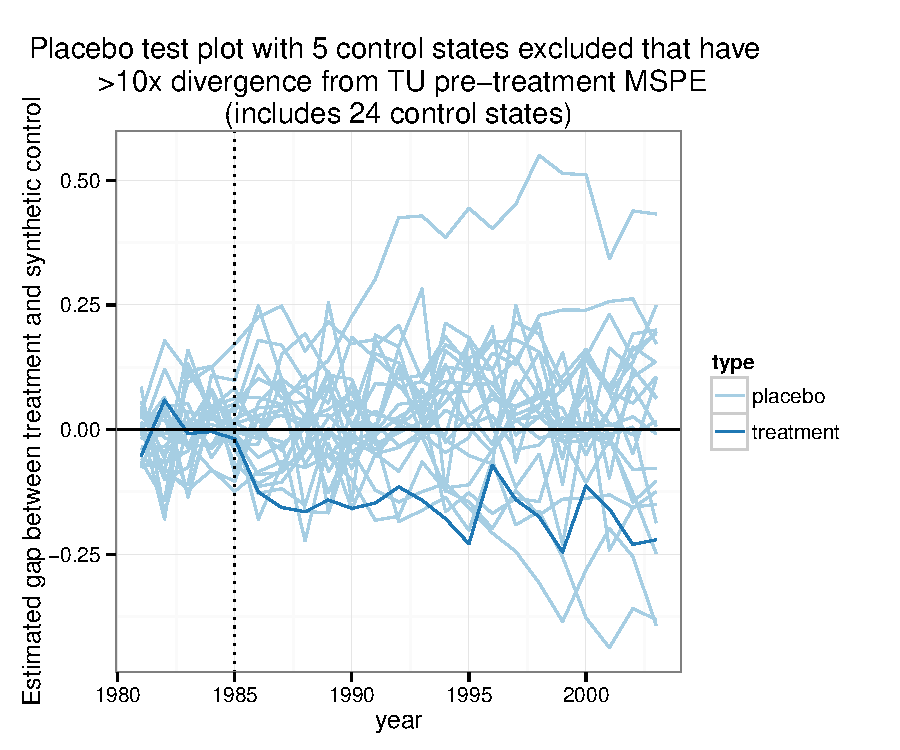
\includegraphics{img-placeboTest10.pdf}
\caption{Placebo test results comparing treatment with placebo analysis on all control states.  This plot excludes control states with MSPE in the pre-treatment period greater than 10x the MSPE for the treatment state}
\label{fig:ps10}
\end{center}
\end{figure}

\begin{figure}[htbp]
\begin{center}
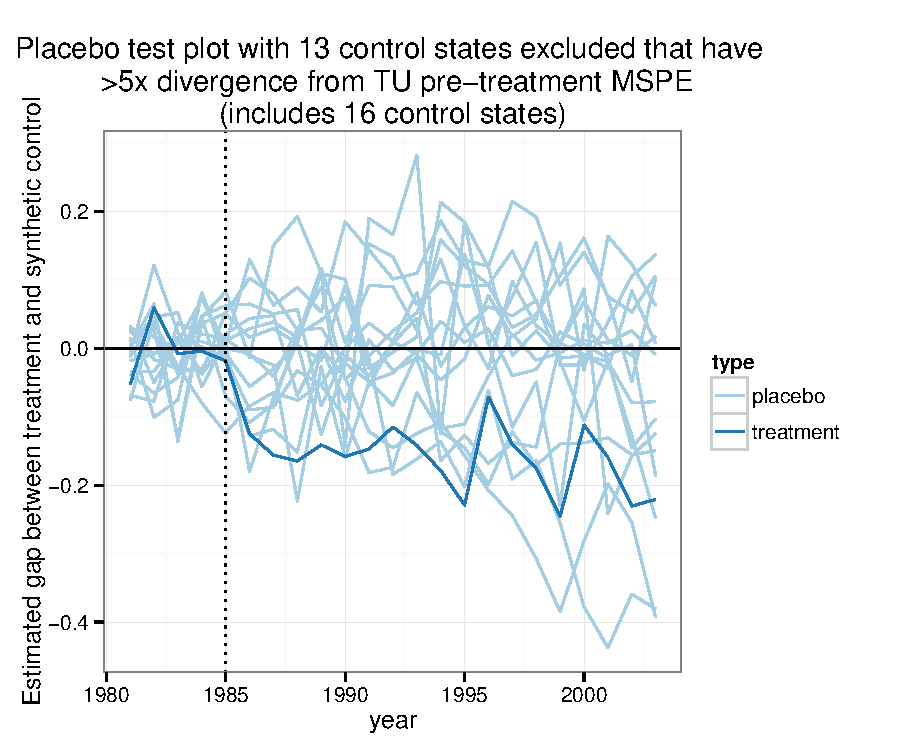
\includegraphics{img-placeboTest5.pdf}
\caption{Placebo test results comparing treatment with placebo analysis on all control states.  This plot excludes control states with MSPE in the pre-treatment period greater than 5x the MSPE for the treatment state}
\label{fig:ps5}
\end{center}
\end{figure}

\begin{figure}[htbp]
\begin{center}
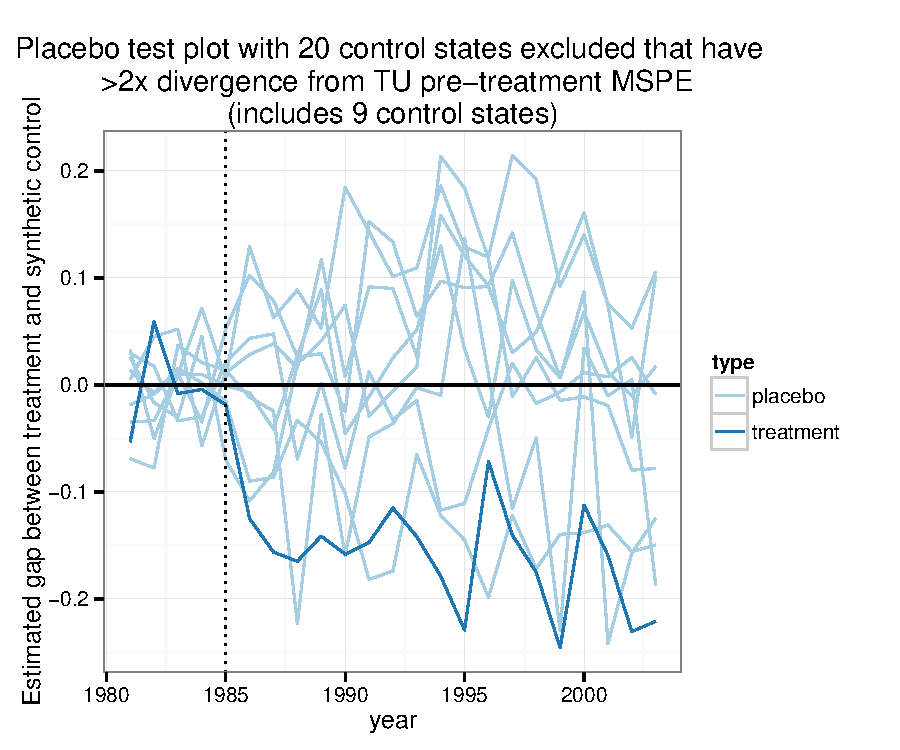
\includegraphics{img-placeboTest2.pdf}
\caption{Placebo test results comparing treatment with placebo analysis on all control states.  This plot excludes control states with MSPE in the pre-treatment period greater than 2x the MSPE for the treatment state}
\label{fig:ps2}
\end{center}
\end{figure}